\documentclass{article}

% set font encoding for PDFLaTeX or XeLaTeX
\usepackage{ifxetex}
\ifxetex
  \usepackage{fontspec}
\else
  \usepackage[T1]{fontenc}
  \usepackage[utf8]{inputenc}
  \usepackage{lmodern}
\fi
\usepackage[top=1in, bottom=1.25in, left=1in, right=1in]{geometry}
% used in maketitle
\title{Evaluacion 1}
\author{Fernando Leyva Cárdenas}

% Enable SageTeX to run SageMath code right inside this LaTeX file.
% documentation: http://mirrors.ctan.org/macros/latex/contrib/sagetex/sagetexpackage.pdf
% \usepackage{sagetex}

\begin{document}
\maketitle

\section{Introducción}
En esta evaluacion se contaran con dos archivos con datos, los cuales son: $sargento-220314.csv$ y Salinidad: $salinidad_sargento-220314.csv$. Esto con el fin de leer, y limpiar dichos datos usando emacs y comandos de linux para despues usar jupyter notebook y poder hacer diagramas de caja, asi como graficas individuales y dobles de las propiedades contenidas en dichos archivos cuyos resultados mostraremos mas adelante.

\section{Desarrollo}
Al descargar los datos, lo primero que hacemos es ir a jupyter notebook, usaremos primero el primer archivo, primeramente debemos leerlo de la siguiente manera:

\begin{verbatim}
# Lee un archivo de texto con la función Pandas "read_csv", con elementos separados por mas de 
# un espacio, brincándose 4 renglones del inicio (encabezados)
df0 = pd.read_csv('sargento_201117.csv', skiprows=1, sep=',')
# "Shift + Enter"
\end{verbatim}
Esto por supuesto despues de importar las librerias necesarias para nuestro trabajo; posteriormente debemos convertir nuestras fechas en una variable temporal suponiendo que leyó bien nuestros datos, para ello usamos el siguiente codigo:

\begin{verbatim}
# Convertir la cadena de caracteres 'Date' en variable temporal 'NDate'
df['Ndate'] = pd.to_datetime(df['Fecha'], format='%m/%d/%Y %H:%M:%S')
df['month'] = df['Ndate'].dt.month
df.head()
\end{verbatim}
Obtenemos como resultado algo asi:

\begin{verbatim}
	#	Fecha	Pres	Temp	WaterLevel	Ndate	month
0	1	10/26/2017 13:00:00	105.612	24.448	-0.150	2017-10-26 13:00:00	10
1	2	10/26/2017 13:15:00	105.513	24.351	-0.160	2017-10-26 13:15:00	10
2	3	10/26/2017 13:30:00	105.433	24.351	-0.168	2017-10-26 13:30:00	10
3	4	10/26/2017 13:45:00	105.385	24.351	-0.173	2017-10-26 13:45:00	10
4	5	10/26/2017 14:00:00	105.321	24.351	-0.179	2017-10-26 14:00:00	10
\end{verbatim}
Incluso podemos ver como los leyó pandas:
\begin{verbatim}
#                      int64
Fecha                 object
Pres                 float64
Temp                 float64
WaterLevel           float64
Ndate         datetime64[ns]
month                  int64
dtype: object
\end{verbatim}

Teniendo listos nuestros datos, podemos graficar boxplots, por ejemplo una boxplot de tiempo contra presion:
\begin{figure}[h]
\centering
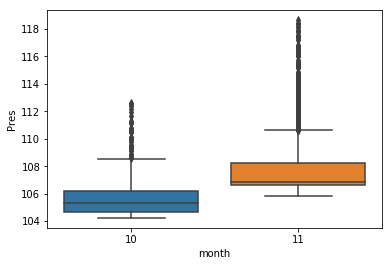
\includegraphics[width=0.65\textwidth]{30.png}
\end{figure}

Ahora con la temperatura:
\begin{figure}[h]
\centering
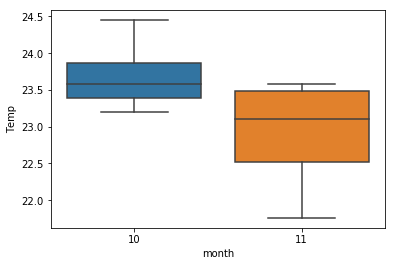
\includegraphics[width=0.65\textwidth]{31.png}
\end{figure}
\newpage
Y con el nivel del agua:
\begin{figure}[h]
\centering
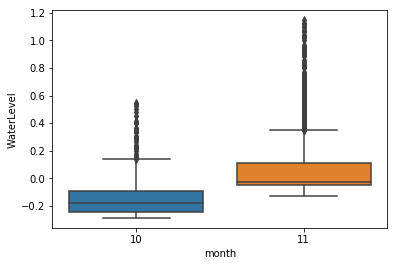
\includegraphics[width=0.65\textwidth]{32.png}
\end{figure}

Ahora, utilizando de nuevo los dos archivos, se hacen los mismos primeros pasos, de importar las librerias necesarias, hacer una variable temporal, etc.
\begin{figure}[h]
\centering
\includegraphics[width=0.57\textwidth]{l.png}
\end{figure}

\newpage
y tambien temperatura contra salinidad, la cual es:
\begin{figure}[h]
\centering
\includegraphics[width=0.57\textwidth]{o.png}
\end{figure}

Tenemos tambien lo que son el comportamiento de una variable, en nuestro caso graficas primero del nivel del mar, la cual es:

\begin{figure}[h]
\centering
\includegraphics[width=0.57\textwidth]{k.png}
\end{figure}

\newpage
Ahora veremos la grafica de la salinidad:

\begin{figure}[h]
\centering
\includegraphics[width=0.57\textwidth]{n.png}
\end{figure}

Ademas tambien producimos la grafica del comportamiento de la temperatura, la cual quedó:

\begin{figure}[h]
\centering
\includegraphics[width=0.57\textwidth]{v.png}
\end{figure}

\newpage
Cada una con su debido comportamiento, ahora lo que hicimos fue graficar dos propiedades, este fue el caso de la temperatura y el nivel del agua, cuyo comportamiento se indica en la siguiente grafica:

\begin{figure}[h]
\centering
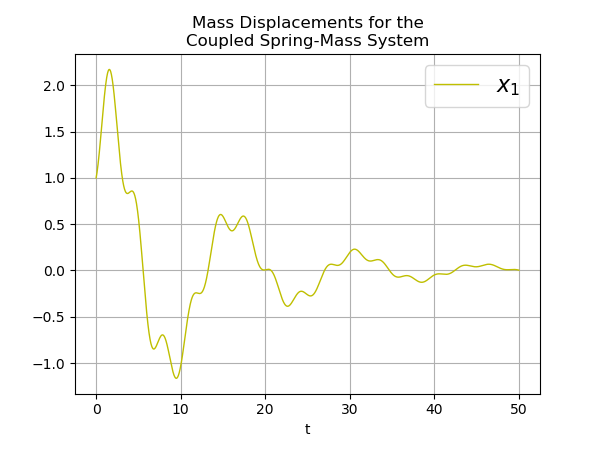
\includegraphics[width=0.57\textwidth]{c.png}
\end{figure}

\section{Conclusión}
Lo que podemos decir de conclusion en esta evaluacion ha sido el aprendizaje al usar jupyter notebook para el analisis de datos, dado que con dichos archivos se pueden explorar y analizar varios factores como fue nuestro caso al estudiar el conportamiento de la salinidad, nivel del agua, temperatura, presion, utilizando el lenguaje de programacion phyton 3.

\end{document}
